
\documentclass{exam}

\usepackage{graphicx}
\usepackage[fleqn]{amsmath}
\usepackage{unitsdef} 
\usepackage{cancel}
\usepackage{float}
\usepackage{mdwlist}
\usepackage{booktabs}
\usepackage{cancel}
\usepackage{polynom}
\usepackage{caption}
\usepackage{fullpage}
\usepackage{enumerate}
% \usepackage{parskip}

% \newcommand{\degree}{\ensuremath{^\circ}} 
\everymath{\displaystyle}

\newunit{\inch}{in}
\newunit{\foot}{ft}
\newunit{\cemtimeter}{cm}

% \begin{figure}[H]
%   \centering
%   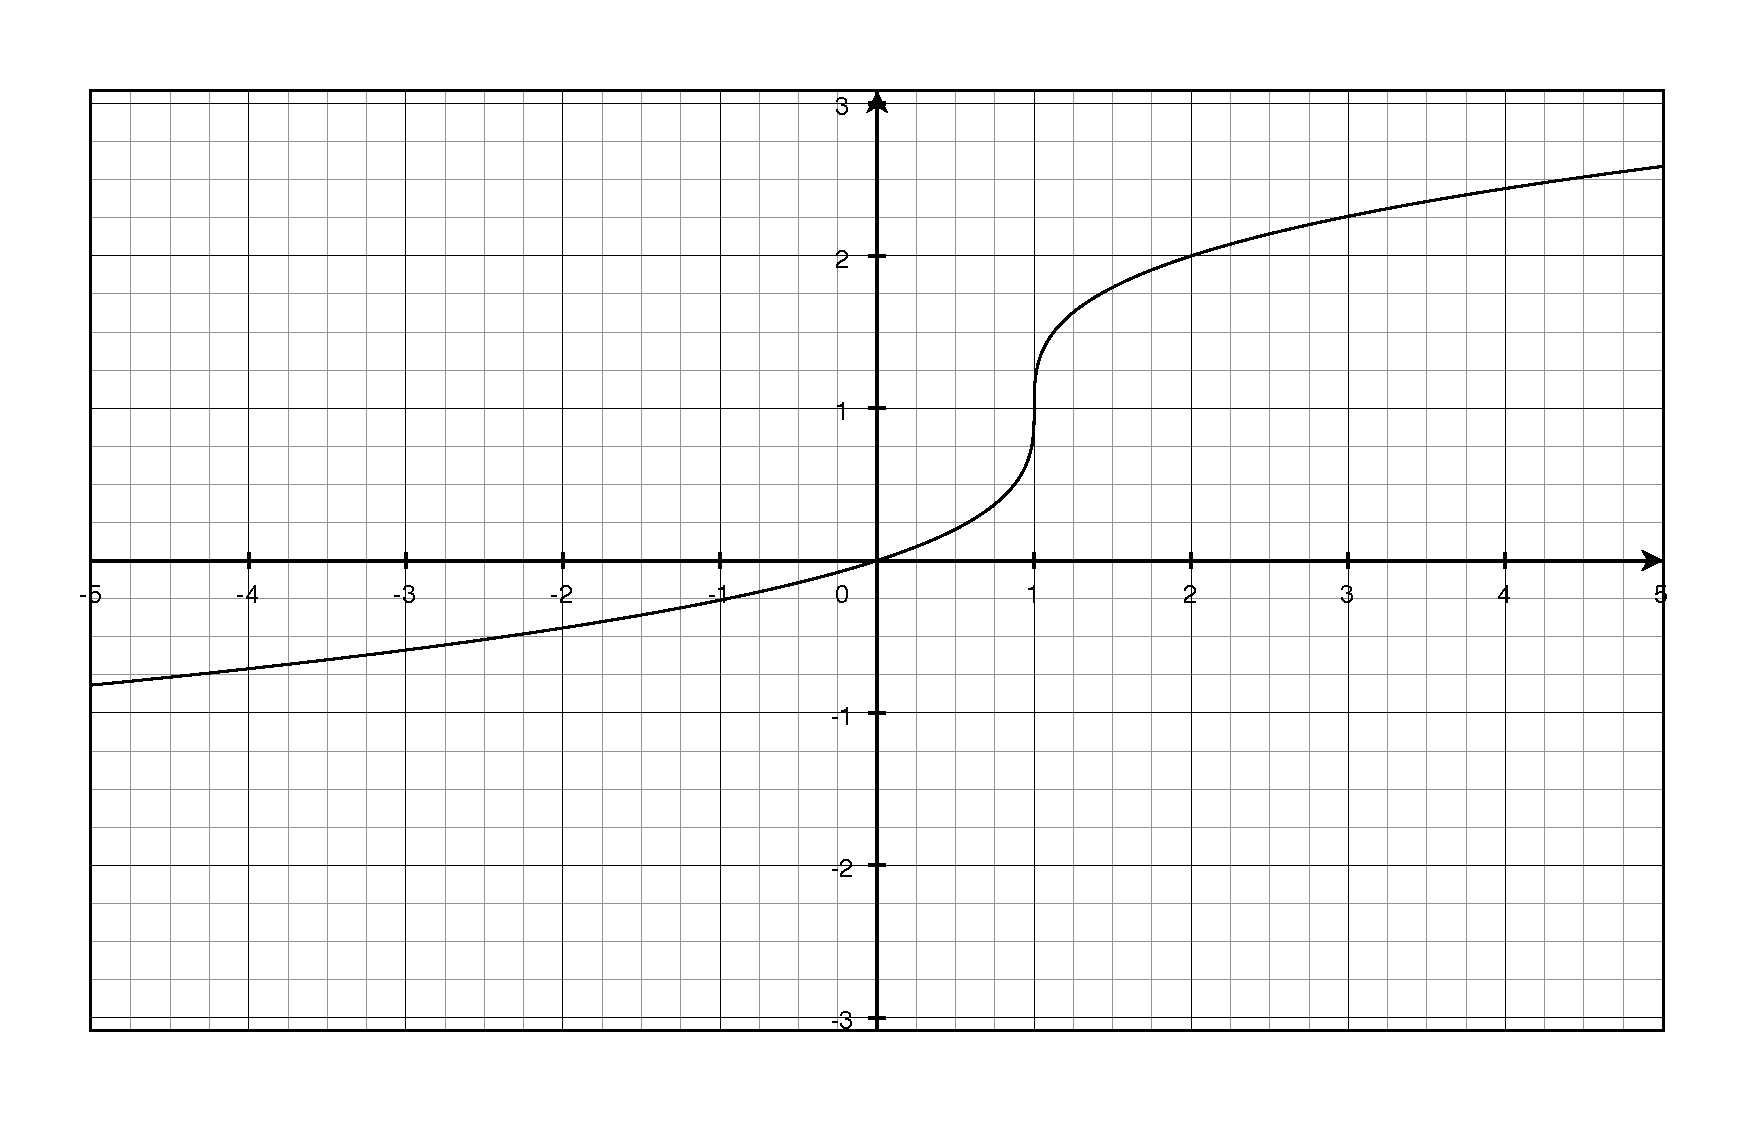
\includegraphics[scale=.3]{question7.eps}
%   \caption*{Question 7}
% \end{figure}

% \begin{tabular}{cc}
% \toprule
% period & amplitude \\
% \midrule
%   $\pi$ & $2$ \\
% \bottomrule
% \end{tabular}

% \printanswers

\ifprintanswers 
\usepackage{2in1, lscape} 
\fi

\title{Math 263B \\ Homework Fourteen}
\date{December 20, 2012}

\begin{document}

\maketitle

\section{Homework}

\begin{itemize*}
  \item Read Section 7.6-7.8
  \item pp 370-372: 1-8, 13-31
  \item pp 377-379: 1-2, 5-8, 11, 13
\end{itemize*}

\ifprintanswers
\pagebreak
\fi

\section{Extra Credit}
page 371, problem 44

\ifprintanswers
\begin{solution}
Solve for x:
\begin{align*}
  y &= \frac{a^x - 1}{a^x + 1} \\
  a^x &= \frac{y + 1}{1 - y} \\
  x &= \log_a \left( \frac{y + 1}{1 - y} \right) \\
\\
  f^{-1}(x) &= \log_a \left( \frac{x + 1}{1 - x} \right) \\
\end{align*}

check:
\begin{align*}
  f(f^{-1}(x)) &= \frac{\cfrac{x + 1}{1 - x} - 1}{\cfrac{x + 1}{1 - x} + 1} = x \\
  f^{-1}(f(x)) &= \log_a \left( \frac{\left( \cfrac{a^x - 1}{a^x + 1} + 1 \right)}{\left(1 - \cfrac{a^x - 1}{a^x + 1} \right)} \right) = x \\
\end{align*}

\end{solution}

\section{Section 7.4}

\begin{description}
\item[1]
\begin{align*}
  x &= \log_2 8 \\
  x &= 3 \\
\end{align*}

\item[2]
\begin{align*}
  \log_5 x &= 2 \\
  x &= 25 \\
\end{align*}

\item[3]
\begin{align*}
  \log_4 x &= \frac{3}{2} \\
  x &= 4^{3/2} \\
    &= 8
\end{align*}

\item[4]
\begin{align*}
  \log_x 64 &= 4 \\
  x^4 &= 64 \\
  x  &= \sqrt[4]{64}
\end{align*}

\item[5]
\begin{align*}
  2 \log_9 \left( \frac{x}{3} \right) &= 1 \\
  \log_9 \left( \frac{x}{3} \right) &= \frac{1}{2} \\
  \frac{x}{3} &= 9^{1/2} \\
%  \frac{x}{3} &= 3 \\
  x &= 9 \\
\end{align*}

\item[6]
\begin{align*}
  \log_4 \left( \frac{1}{2x} \right) &= 3 \\
  \frac{1}{2x} &= 4^3 \\
  x &= \frac{1}{128} \\
\end{align*}

\item[7]
\begin{align*}
  \log_2 (x + 3) - \log_2 x &= 2 \\
  \log_2 \left( \frac{x + 3}{x} \right) &= 2 \\
  \frac{x + 3}{x} &= 2^2 \\
  % x + 3 &= 4x \\
  x &= 1 \\
\end{align*}

\item[8]
\begin{align*}
  \log_5 (x + 3) - \log_5 x &= 1 \\
  \log_5 \left( \frac{x + 3}{x} \right) &= 1 \\
  \frac{x + 3}{x} &= 4 \\
  x + 3 &= 5x \\
  x &= \frac{3}{4} \\
\end{align*}

\item[13]
\begin{align*}
  2^x &= 17 \\
  x &= \log_2 17 \\
    &= \frac{\ln 17}{\ln 2} \\
    &\approx 4.0875 \\
\end{align*}

\item[14]
\begin{align*}
  5^z &= 13 \\
  z &= \log_5 13 \\
    &= \frac{\ln 13}{\ln 5} \\
    &\approx 1.5937 \\
\end{align*}

\item[15]
\begin{align*}
  5^{2s - 3} &= 4 \\
  2s - 3 &= \log_5 4 \\
  2s &= 3 + \log_5 4 \\
  s &= \frac{3 + \log_5 4}{2} \\
    &\approx 1.9307 \\
\end{align*}

\item[16]
\begin{align*}
  12^{1/(\theta - 1)} &= 4 \\
  \frac{1}{\theta - 1} &= \log_12 4 \\
  \theta - 1 &= \frac{1}{\log_12 4} \\
  \theta &= 1 + \frac{1}{\log_12 4} \\
         &\approx 2.7925 \\
\end{align*}

\item[17]
\begin{align*}
  D_x 6^{2x} &= 6^{2x} \cdot \ln 6 \cdot 2
\end{align*}

\item[18]
\begin{align*}
  D_x 3^{2x^2 - 3x} &= 3^{2x^2 - 3x} \cdot (4x - 3)
\end{align*}

\item[19]
\begin{align*}
  D_x \log_3 e^x &= D_x x \log_3 e \\
  &= \log_3 e \\
\end{align*}

\item[20]
\begin{align*}
  D_x \log_{10} (x^3 + 9) &= \frac{3x^2}{\ln 10 \cdot (x^3 + 9)}
\end{align*}

\item[21]
\begin{align*}
  D_x \left[ 3^x \ln(x + 5) \right] &= \frac{3^x}{x + 5} + \ln(x + 5) \cdot 3^x \cdot \ln 3 \\
  &= 3^x \left( \frac{1}{x + 5} + \ln 3 \cdot \ln(x + 5) \right) \\
\end{align*}

\item[22]
\begin{align*}
  D_{\theta} \sqrt{ \log 3^{\theta^2 - \theta}} &=  D_{\theta} [ (\log 3^{\theta^2 - \theta})^{1/2} ] \\
    &= \frac{1}{2} \cdot [ \log (3^{\theta^2 - \theta}) ]^{-1/2} \cdot D_{\theta} \log \left(3^{\theta^2 - \theta}\right) \\
    &= \frac{1}{2 \sqrt{ \log 3^{\theta^2 - \theta}}} \cdot  D_{\theta} [  (\theta^2 - \theta) \cdot \log 3 ] \\
    &= \frac{\log 3 \cdot D_{\theta} (\theta^2 - \theta)}{2 \sqrt{\log \left(3^{\theta^2 - \theta}\right)}}  \\
    &= \frac{\log 3 \cdot (2\theta - 1)}{2 \sqrt{\log \left(3^{\theta^2 - \theta}\right)}}  \\
\end{align*}

\item[23]
\begin{align*}
  u &= x^2 \\
  du &= 2 x \, dx
\\
  \int x 2^{x^2} \, \mathrm{d}x &= \frac{1}{2} \int 2^u \, \mathrm{d}u \\
  &= \frac{1}{2} \left( \frac{2^u}{\ln 2} + C \right) \\
  &= \frac{2^u}{2 \cdot \ln 2} + C \\
  &= \frac{2^{x^2}}{2 \cdot \ln 2} + C \\
\end{align*}

check: $D_x \left( \frac{2^{x^2}}{2 \cdot \ln 2} \right) = x 2^{x^2}$

\item[24]
\begin{align*}
  u &= 5x - 1 \\
  du &= 5 \, dx
\\
  \int 10^{5x - 1} \, \mathrm{d}x &= \frac{1}{5} \int 10^u \, \mathrm{d}u \\
  &= \frac{10^u}{5 \cdot \ln 10} + C \\
  &= \frac{10^{5x - 1}}{5 \cdot \ln 10} + C \\
\end{align*}

check: $D_x \left( \frac{10^{5x - 1}}{5 \ln 10} \right) = 10^{5x - 1}$

\item[25]
\begin{align*}
  u &= x^{1/2} \\
  du &= \frac{dx}{2 \sqrt{x}} \\
  u(1) &= 1 \\
  u(4) &= 2 \\
\\
  \int_1^4 \frac{5^{\sqrt{x}}}{\sqrt{x}} \, \mathrm{d}x &= 2 \int_1^2 5^u \, \mathrm{d}u \\
  &= \frac{2 \cdot 5^u}{\ln 5} \bigg|_1^2 \\
  &= \frac{40}{\ln 5} \\
\end{align*}

\item[26]
\begin{align*}
  u &= 3x \\
  du &= 3 \, dx\\
  u(0) &= 0 \\
  u(1) &= 3 \\
\\
  \int_0^1 (10^{3x} + 10^{-3x} \, \mathrm{d}x &= \frac{1}{3} \int_0^3 (10^u + 10^{-u} \, \mathrm{d}u \\
  &= \frac{1}{3 \cdot \ln 10} \cdot \left(10^u + 10^{-u} \right|_0^3 \\
  &= \frac{1000.001}{3 \cdot \ln 10} \\
\end{align*}

\item[27]
\begin{align*}
  y &= 10^{x^2} + (x^2)^{10} \\
    &= 10^{x^2} + x^{20} \\
  y' &= 10^{x^2} \cdot \ln 10 \cdot 2x + 20x^{19} \\
\end{align*}

\item[28]
\begin{align*}
  y &= \sin^2 x + 2^{\sin x} \\
  y' &= 2 \sin x \cos x + 2^{\sin x} \cdot \ln 2 \cdot \cos x \\
\end{align*}

\item[29]
\begin{align*}
  y &= x^{\pi + 1} + (\pi + 1)^x \\
  y' &= (\pi + 1)x^{\pi} + (\pi + 1)^x \ln(\pi + 1) \\
\end{align*}

\item[30]
\begin{align*}
  y &= 2^{e^x} + (2^e)^x \\
    &= 2^{e^x} + 2^{ex} \\
  y' &= 2^{e^x} \cdot \ln 2 \cdot e^x + 2^{ex} \cdot \ln 2 \cdot e \\
     &= e \ln 2 (2^{e^x} \cdot e^{x - 1} + 2^{ex} ) \\
\end{align*}

\item[31]
\begin{align*}
  y &= (x^2 + 1)^{\ln x} \\
  \ln y &= \ln (x^2 + 1)^{\ln x} \\ 
        &= \ln x \cdot \ln (x^2 + 1) \\
  \frac{y'}{y} &= \frac{\ln(x^2 + 1)}{x} + \frac{2x \ln x}{x^2 + 1} \\
  y' &= (x^2 + 1)^{\ln x} \cdot \left( \frac{\ln(x^2 + 1)}{x} + \frac{2x \ln x}{x^2 + 1} \right) \\
\end{align*}

\end{description}
\else

% Law never made men a whit more just; and, by means of their respect for it, even the well-disposed are daily made the
% agents of injustice (thoreau)

\vspace{9 cm} 

{\em I heartily accept the motto, ``That government is best which governs least''; and I should like to see it acted up
  to more rapidly and systematically. Carried out, it finally amounts to this, which also I believe---``That government
  is best which governs not at all''; and when men are prepared for it, that will be the kind of government which they
  will have.}

\vspace{0.1 cm}
\hspace{0.5 cm} --Henry David Thoreau

\fi

\end{document}

